\documentclass[a4paper,3p,sort&compress]{elsarticle}

\usepackage[draft]{hyperref}
\usepackage{url}
\usepackage{booktabs}
\usepackage{graphicx}
\usepackage{xspace}
\usepackage{booktabs}
\usepackage{makecell}
\usepackage{lineno}
\usepackage{natbib}
\usepackage{amsmath}
\DeclareRobustCommand{\citeext}[1]{\citeauthor{#1}~\cite{#1}}

\usepackage[nomargin,inline,draft]{fixme}
\fxsetup{theme=color,mode=multiuser}
\FXRegisterAuthor{j}{jla}{\color{purple}JLA}
\FXRegisterAuthor{s}{spv}{\color{teal}SPV}

\journal{-}

%% `Elsevier LaTeX' style
\bibliographystyle{plain}
%%%%%%%%%%%%%%%%%%%%%%%

\begin{document}
\linenumbers

% Macro para escribir NO$_2$
\newcommand{\no}{NO\textsubscript{2}\xspace}
% Macro for superscript
\newcommand{\ts}{\textsuperscript}

\begin{frontmatter}

  \title{Introducing a novel visualization technique for time series uncertainty visualization}


  \author{Sebasti\'an P\'erez Vasseur}
  \author{Jos\'e L. Aznarte}
  \address{Artificial Intelligence Department\\Universidad Nacional de
    Educaci\'on a Distancia --- UNED\\c/ Juan del Rosal, 16, Madrid, Spain}
  \ead{jlaznarte@dia.uned.es}


\begin{abstract}

There are few studies dealing with visualization techniques applied to uncertainty in time series, 
where the evolution of uncertainty over time is relevant. After reviewing the existing
literature on the field, we found 3 visualization techniques we could apply to
this case: the gradient chart, the box plot, and the confidence interval charts.
We also applied the frequency framing technique to design a fourth and novel way 
to visualize uncertainty in time series: the natural frequency chart. We compared those charts 
against a predefined set of metrics around the user's ability to estimate the outcome 
probabilities at certain times (accuracy, time to read, confidence and, perceived difficulty) 
and we devised a social experiment through Amazon Mechanical Turk to evaluate the different charts. 
From the results of our experiments, we can conclude that the application of natural 
frequencies does indeed provide better readability than any of the alternatives.

\end{abstract}

\begin{keyword}
probabilistic forecasting \sep visualization \sep natural frequency chart
\end{keyword}

\end{frontmatter}

%\linenumbers

\section{Introduction}
\label{sec:intro}

During all the stages of data analysis and modelling, practitioners are
confronted with uncertainty, which can have several causes such as missing
information, statistical errors, or modeling approximations, and which has
important implications for the modelling process. This also affects time series
forecasting models, whose regressors and estimations are naturally subject to
some degree of uncertainty. The latest M competition \cite{makridakis_m5_2022}, 
aiming to advance the 
theory and practice of time series forecasting has now an "uncertainty" 
mode confirming uncertainty is becoming an important topic. In any case, 
it is always beneficial to take into
account uncertainty when making decisions as it helps estimate the risks and
rewards that can be expected (Padilla et al. \cite{padilla_uncertainty_2021}).
For example, Rouston et al. \cite{roulston_laboratory_2006} revealed how
analysts took better decisions from temperature forecasts when taking
uncertainty into account. 

One way to model uncertainty is through the use of a probability distribution
which indicates the probability of the different outcomes of the target
variable. In that sense, probabilistic forecasting is a set of techniques
designed to produce forecasting models that are able to predict such probability
distributions instead of single valued predictions. For example, Pinson et al.
\cite{pinson_non-parametric_2007} showed how probabilistic forecasting in wind
energy optimized the use of this natural resource. Also regarding air
quality forecasting, \cite{vasseur_comparing_2021} indicated how probabilistic
forecasting enabled the estimation of the future risk of a pollutant surpassing
a certain regulatory threshold.

However, there is a concern that the public will not be able to understand
predictions that come with a measure of their uncertainty. This fear is
reinforced by cases where tools to communicate uncertainty seem to confuse the
users. For example, Belia et al \cite{belia_researchers_2005} showed that even
leading researchers had trouble reading error bars. As Padilla et al.
\cite{padilla_uncertainty_2021} points out, this could be due to either the
abstract nature of the probability concepts or to poor communication techniques.

One way to improve the communication of uncertainty is based on data
visualization. For instance, Perez Cota et al. \cite{cota_importance_2014}
mentioned how analytical tools in the business environment are embracing data
visualizations to provide a better view of the data. Indeed, as stated by Islam
et al. \cite{islam_overview_2019}, visualizations are easier for the human brain
to intuitively understand and process.

With a good visualization, it is easier to have a qualitative understanding of
the uncertainty of the target variable. However, in some cases, it is even more
important to be able to quantitatively estimate this uncertainty as it helps
estimate precisely the risks and rewards stemming from the decision process.

As pointed out by Weiskopf et al. \cite{weiskopf_uncertainty_2022} or Padilla et
al. \cite{padilla_uncertainty_2021}, uncertainty visualization has motivated
research in recent years. However, this research on uncertainty visualization
usually consists of the classification of visualization techniques for
uncertainty, and few works have measured the reading accuracy of those.
Furthermore, as pointed out by Leffrang et al. \cite{leffrang_should_2021},
there's little research on uncertainty visualization applied to time series and
especially time series forecasting. Indeed, time series forecasting presents an
additional challenge as it requires a presentation of the evolution of the
uncertainty in a relatively small visualization area.

Following this thought, this paper will attempt to fill this gap by applying
different visualization techniques to time series uncertainty and will compare
those methods against the question: how well can we estimate the outcome
probabilities with it? We will present in Section 2 the current research on
uncertainty visualization. We will then, in Section 3, present different
solutions and use them to visualize the uncertainty around the predictions of a
Probabilistic time series forecasting model and in Sections 4 and 5, inspired by
Brennen et al. \cite{brennen_instrument_2018}, we will propose a social
experiment which will allow to compare those charts in terms of probability
reading difficulty.

In order to set up a realistic environment, we will use as an application ground
for this comparison a probabilistic forecast of \no~concentrations in the city
of Madrid. This forecast contains the full predicted distribution of \no~levels
over time and each studied chart will display this very same time series with
uncertainty.

\section{State of the art}
\label{sec:results}

As noted by Joslyn et al. \cite{joslyn_communicating_2010}, the shortcomings in
uncertainty visualization lead to a new surge of research in visualization
techniques. Pang et al. \cite{pang_approaches_1997} were the first to gather
uncertainty visualization techniques and classify them to bring order to the
field and help practitioners choose the right visualization. However, their
taxonomy did not explain how the visualization works nor helped create new ones.

Following uncertainty visualization surveys were based on data types (Potter et
al. \cite{potter_quantification_2012} and Brodlie et al.
\cite{brodlie_review_2012}), sources of uncertainty (Bonneau et al.
\cite{bonneau_overview_2014}), types of uncertainty (Ristovski et al.
\cite{ristovski_uncertainty_2014}). Jena et al. \cite{jena_uncertainty_2020}
classified the techniques based on the publication channel and audience and even
made their findings available online as a public website.

The most notable work is the classifications delivered by Padilla et al.
\cite{padilla_uncertainty_2021} which classifies according to the type of visual
mapping. They provide the main types of uncertainty visualization techniques
with their shortcomings and explain that there's no one-size-fits-all solution
and that visualization techniques must be chosen in consideration to their use
case.

Following that work, one of the most typical approaches represent visual
boundaries such as isocontours and error bars to display value areas within a
certain confidence interval. The problem with this approach is that individuals
may exclude as impossible values that lie outside the confidence interval, while
those values are still possible, only less probable. Also, as stated previously,
Belia et al \cite{belia_researchers_2005} showed that even leading researchers
had trouble reading error bars as they confused standard errors and confidence
intervals. In addition, Joslyn and LeClerc \cite{joslyn_decisions_2013} showed
that individuals could also be inclined to take uncertain information as
deterministic, for example by considering the confidence interval of a
temperature forecast as high and low temperatures.

One possible solution to this problem is the use of so-called HOPs (hypothetical
outcome plots) \cite{padilla_uncertainty_2021}. HOPs sequentially display random
values from a distribution in an animation. However, this technique can not be
applied to static visualizations and requires media formats like video or
animated images: This makes the diffusion of that type of visualization more
difficult.

An alternative approach is visual semiotics, which employs visual encodings such
as fuzziness or color to represent the probability of a certain value. An
example of this would be the use of gradients to represent the full probability
distribution. Nevertheless, this type of encoding makes it difficult to read
specific values.

Finally, frequency framing uses natural frequencies to display probabilities. As
noted by Gerd Gigerenzer \cite{gigerenzer_psychology_1996}, individuals prefer frequencies
or ratios, like 1/10, when confronted to understanding probability. This has led
to the development of the quantile dot plot, for example. This plot, created by
Kay et al. \cite{2016-when-ish-is-my-bus}, represents the probability
distribution with dots: by using 20 dots, each would represent 1/20 probability
and they are placed according to the quantiles of the distribution. Quantile dot
plots have proved to lead to better distribution understanding and probability
estimate reading.

However those approaches do not address specifically the problem of uncertainty
in time series and, as pointed out by Leffrang et al.
\cite{leffrang_should_2021}, not much research has been applied to this field.
Indeed, as stated previously, this is challenging as the visualizations would
need to show the evolution of uncertainty in time in a relatively constrained
space. Of course, for this problem one could apply some of the solutions
described above such as confidence interval charts or box plots (visual
boundaries) or gradient charts (visual semiotics). However, to the best of our
knowledge, a solution involving frequency framing is yet to be proposed.

Furthermore, most of the existing research concentrates on providing exhaustive
lists of uncertainty visualization techniques and does not focus on the user's
ability to read them. There are notable exceptions like the research by Kay et
al. \cite{2016-when-ish-is-my-bus} on the uncertainty of waiting times or
Brennen et al. \cite{brennen_instrument_2018}, who developed an approach to
evaluate uncertainty visualizations. Leffrang et al. \cite{leffrang_should_2021}
paper is the only example applied to time series forecasting uncertainty.

As noted by Cleveland et al. \cite{cleveland_graphical_1984} the basic
methodology to compare visualizations is to measure how accurate is the decoding
of the information enclosed therein: comparing the value encoded in the
visualization with the value read by the user. In their classic paper, Cleveland
et al. \cite{cleveland_graphical_1984} produced a ranking of visual encodings
for numerical values with the position being the most accurate encoder. However,
as noted by Brennen et al. \cite{brennen_instrument_2018}, more complex
visualizations could lead to better readability but would also require longer
times to read the chart. Also, they noted that those measures do not take into
account the perception of the user, especially when the visualization is showing
uncertainty. Therefore they developed a methodology to systematically evaluate
the performance of uncertainty visualizations, based on four measures: cognitive
load, confidence, reading error, and time to read. Those metrics will be used in
Section 4 to compare the different visualization techniques.

\section{Time Series Probabilistic Charts}
\label{sec:time_series}

\begin{figure}
  \centering
  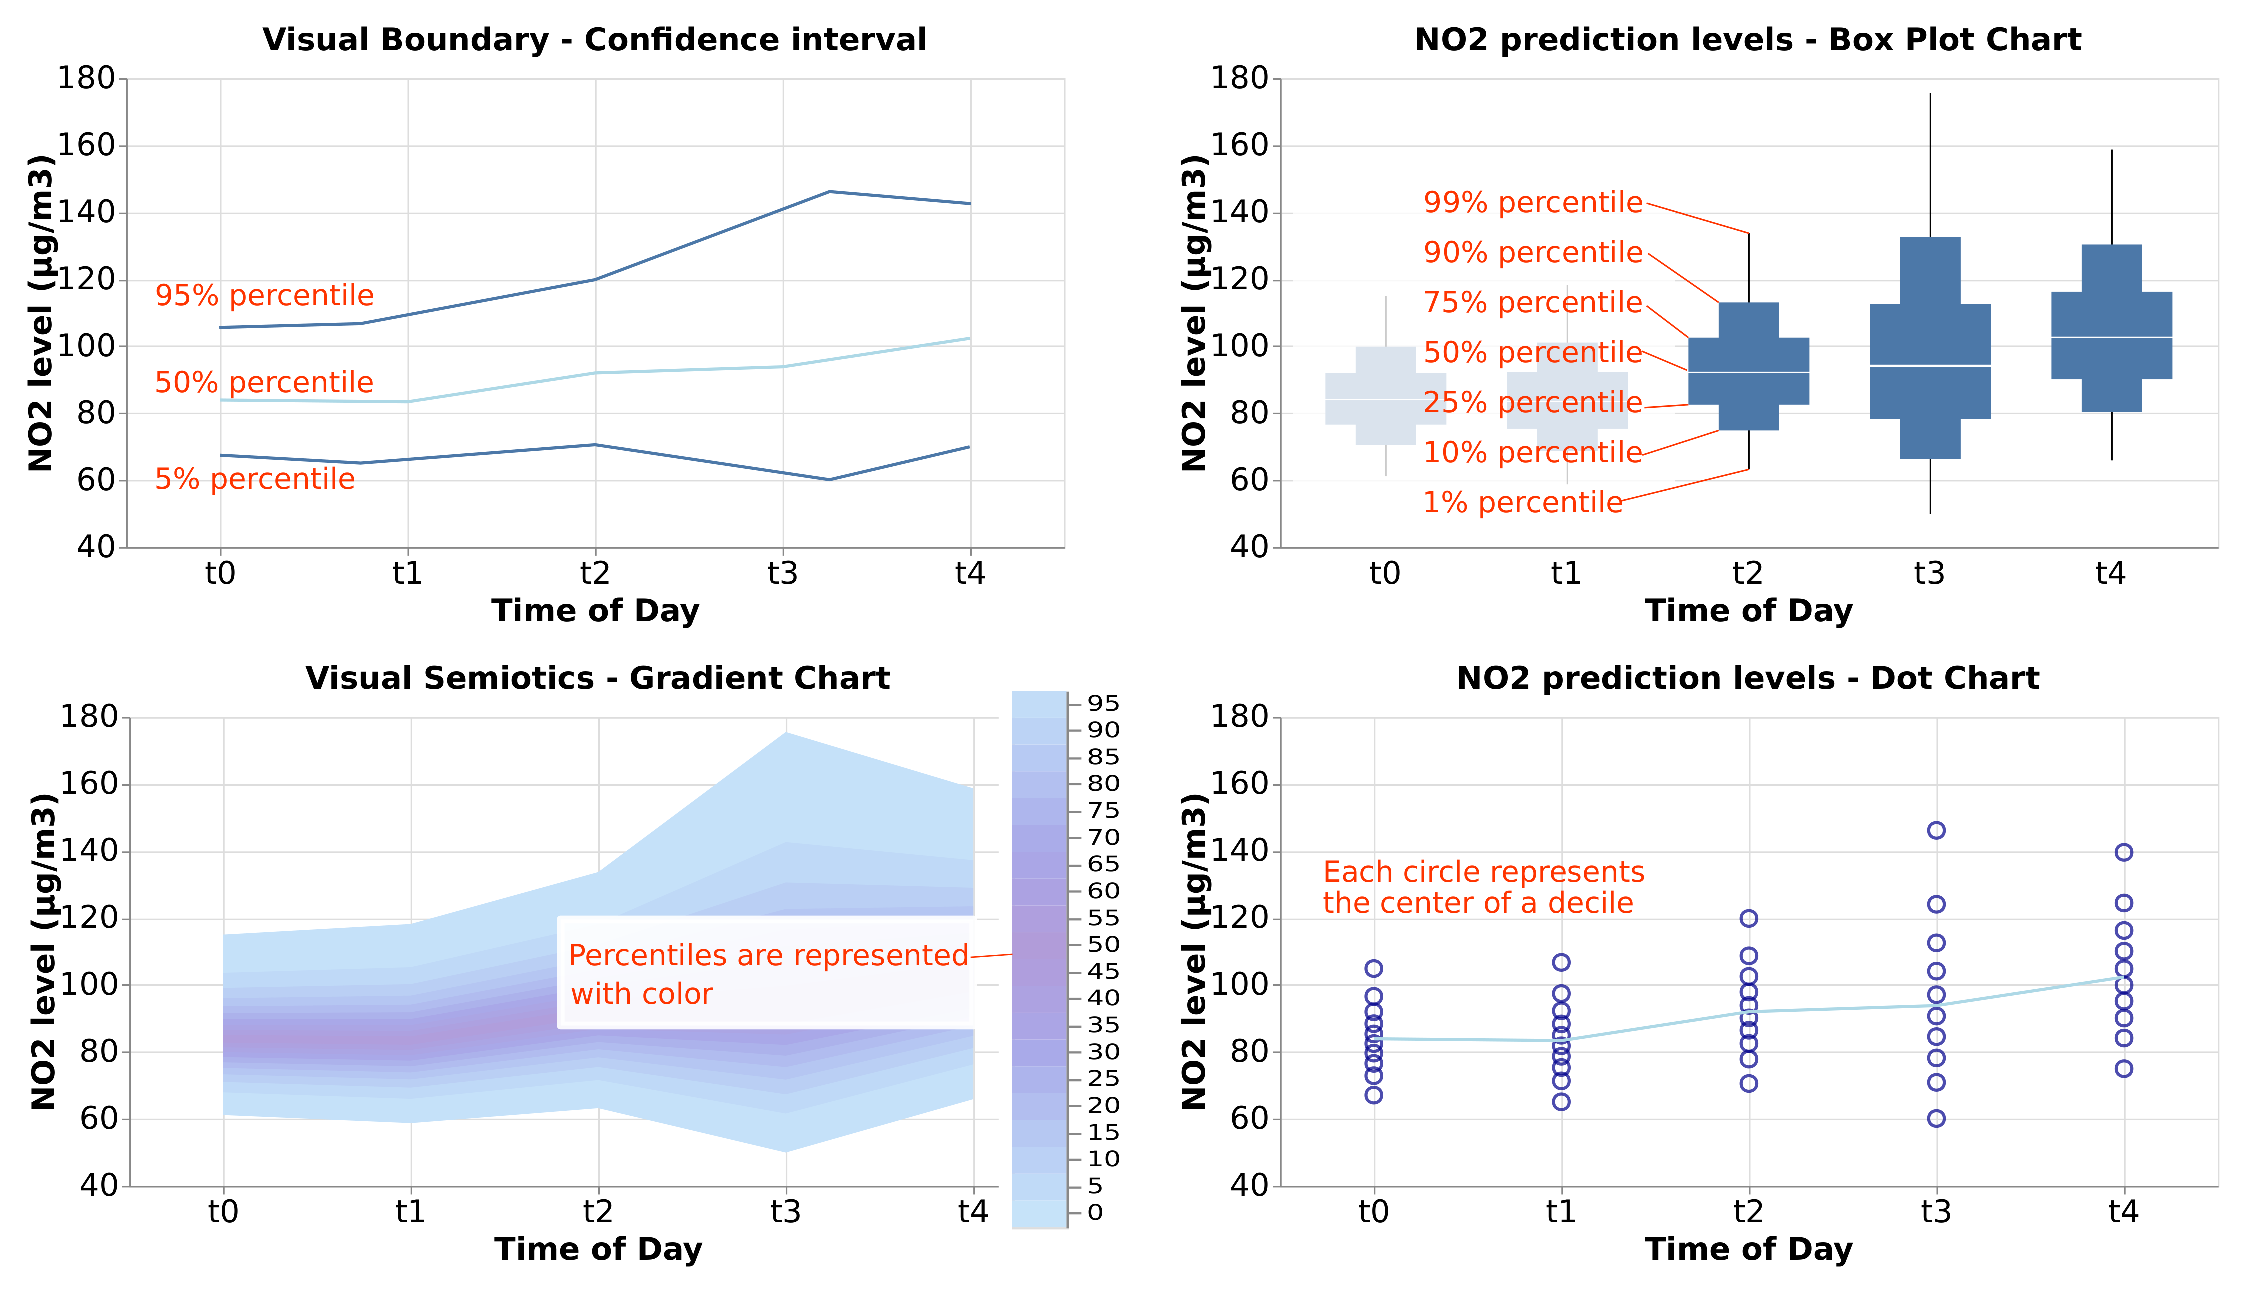
\includegraphics[width=.9\textwidth]{charts_vector}
  \caption{\label{figure:charts} Probabilistic Forecast of \no~concentrations in Madrid
    with different types of time Series Chart. Top Left: Confidence Interval.
    Top Right: Box Plot. Bottom Left: Gradient Chart. Bottom Right: Natural
    Frequency Time Chart.}
\end{figure}

Based on the aforementioned research, we have identified the following charts as
suitable to display uncertainty in time series. Figure \ref{figure:charts} shows
a summary of those time series charts.

The first is the confidence interval chart. This shows the evolution of the
median of the distribution over time with a central line which is flanked by
other two lines representing the evolution of the 5\ts{th} and 95\ts{th}
percentile of the distribution. The user estimates the probabilities with the
distance of the points to those lines.

Secondly, the box plot chart shows different percentiles with “boxes”. For each
point in time, a line shows the location of the mean, then 2 boxes display
different percentiles: the first rectangle (or box) lower and upper parts are
located at the 25\ts{th} and 75\ts{th} percentile respectively, a narrower box
upper and lower parts show the 5\ts{th} and 95\ts{th} percentile and finally a
line’s edges show the 1\ts{st} and 99\ts{th} percentile. This visual boundary
representation shows more percentiles than the confidence interval and is
recommended when the distribution is not symmetrical and to show the edges of
the distribution. An evolution of this chart in meteorology is called EPSgram or
ensemble meteogram, and shows still more quantiles in smaller boxes on top and
below the main one.

The gradient chart shows the evolution of the median with a line and then
displays the different percentiles with overlapping areas whose degraded color
corresponds to the percentile. We end up having an area with a gradient
delimited by 2 lines: the 1\ts{st} and 99\ts{th} percentile. This representation
allows having the full range of percentiles represented.

The 3 methods described above have been used in the literature as a way to
display the overall uncertainty of the target variable. However, they are not
designed for probability readability: they are not so useful, for example, to
determine the probability of the target variable being within a certain range or
above a certain value. Also, each of those methods has its shortcomings. The
confidence interval gives a false sense of determinism as mentioned previously
and values outside the interval may not be taken into account. The confidence
interval is also not a good solution when the distribution of the target
variable has a long tail. The box plot shows only some percentiles and it can be
difficult to estimate the probabilities from the boxes' boundaries. Finally,
although the gradient displays the most information, it has been shown that
color is not a good visual encoding and is more difficult to read than other
encodings \cite{cleveland_graphical_1984}.

Since none of these solutions was based on natural frequencies for time series,
we decided to apply this idea to this case and design the natural frequency time
chart. While frequency framing has already been used to display uncertainty, the
application of this technique for time series uncertainty visualization is
novel. First, it shows the evolution of the median of the distribution in a
line. And then, for each time step, 10 percentiles from 5\ts{th} to 95\ts{th}
(5\ts{th}, 10\ts{th}, 15\ts{th}, \ldots) are represented: in this way we can estimate
the percentage probability of being in an interval as 10 times the number of
circles in that interval. We have chosen 10 percentiles as it makes it easy to
calculate the probability (just multiply by 10). Also a higher number would have
cramped the chart and made it difficult to view the circles as separate.

\section{Experimental Design}
\label{sec:exp_design}

We compare the charts described in the previous section and displayed in Figure
\ref{figure:charts} in terms of probability reading ease: how well can the
charts communicate the probability that the evolving target is within a certain
interval at a certain time point? For this, we will use as inspiration the
experiments of Brennen et al. \cite{brennen_instrument_2018} and will use
similar metrics as them: reading error, time to answer, cognitive load, and
perception.

The reading error will be estimated as the absolute value of the difference
between the read probability and the real probability. The time to answer will
be calculated from the moment the reader sees the chart until they submit their
answer. The cognitive load and the confidence are the perceived difficulty
reading the charts and the perceived confidence in the accuracy of the answer.
The participant is asked to do a self-assessment on those metrics at the end of
the survey.

We have built a probabilistic time series forecasting model that estimates the
distribution of \no~concentrations in one of the air quality stations deployed
in the city of Madrid, Spain. Those stations continuously measure the level of
certain pollutants like O$_{3}$ or \no and serve as a monitoring tool for the
air quality of the city. If the pollutant reaches certain levels, it can be
dangerous for the city's inhabitants health. Therefore, it becomes necessary for
the city administration to forecast the air quality levels to take decisions
based on it (like limiting car traffic to reduce it beforehand). Our model
produces an hourly forecast for the next day of one of the more dangerous
pollutants: \no. This forecast contains, for each future hour of the day, the
probability distribution of the target variable and therefore provides the
evolution of the probability distribution of the target variable
(\no~concentration).

We will display this very same evolution using each of the four types of charts
and we will evaluate how well users can read the probability of the
\no~concentration being within a certain range at a certain future hour.

For this, we request the participation of users through the Amazon Mechanical
Turk website. This service randomly picks 80 individuals with a minimum skill
set (as proposed by Brennen et al. \cite{brennen_instrument_2018}, we select
Master level participants, who are workers who ''have consistently demonstrated
a high degree of success in performing a wide range of human intelligence tasks
across a large number of requesters'').

We implemented the charts in the python programming language using the Altair
python library \cite{vanderplas2018altair} and saved them as static vector
images for their use in our experiments. The source code is available as
open-source software \cite{Perez-Vasseur_Time_Series_Uncertainty_2022}. 
We then directed the participants
to a website implemented for this experiment: each individual is presented a
single type of chart from the four described above with an explanation of how it
works, then when they consider themselves ready, they are asked to estimate from
the chart five probabilities at five different moments. The questions were:
\begin{itemize}
  \item What is the probability of the \no~concentrations being between 150 and 200 on November 21st at 22:00?
  \item What is the probability of the \no~concentrations being between 70 and 120 on November 21st at 14:00?
  \item What is the probability of the \no~concentrations being above 150 on November 22nd at 09:00?
  \item What is the probability of the \no~concentrations being between 50 and 100 on November 21st at 11:00?
  \item What is the probability of the \no~concentrations being above 200 on November 21st at 20:00?
\end{itemize}

Note that the 1\ts{st}, 2\ts{nd} and 4\ts{th} questions are requesting the
probability of the target variable being in a closed interval, whereas the
3\ts{rd} and 5\ts{th} questions are requesting for an open interval (a value
greater than a threshold). For each question, we measure the accuracy and the
time it took to perform each estimation. Once the individuals have estimated the
probabilities, they are asked how confident they felt and how difficult the task
was considered.

In order to guarantee statistical significance, we tested our hypotheses on 80
individuals: 20 individuals per type of chart and, therefore we would
theoretically have 100 answers per type of chart.

\section{Results}
\label{sec:results}

\begin{figure}
  \centering
  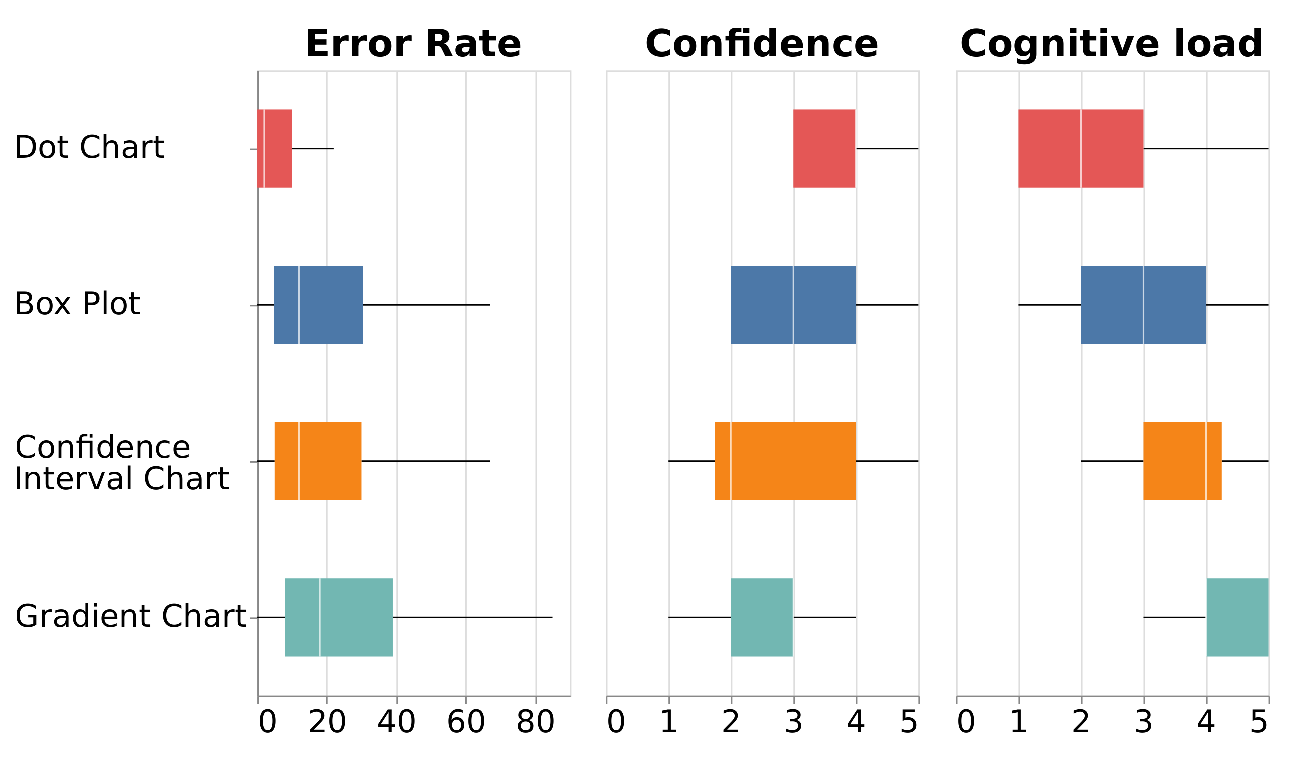
\includegraphics[width=0.8\textwidth]{comparison}
  \caption{\label{figure:errors}Reading Error, confidence, and perceived
    difficulty per type of visualization. The black vertical line represents the
    median. The whiskers represent the 10 and 90 percentile and the box shows
    the 25 and 75 percentile.}
\end{figure}

\begin{table}
  \centering
  \begin{tabular}{lrr}
    \toprule
    {}Question &     Error Mean &        Error Std Deviation \\
    \midrule
    1 &  19.4 &  16.8 \\
    2 &  20.7 &  12.1 \\
    3 &  10.9 &  18.9 \\
    4 &  27.0 &  26.9 \\
    5 &  16.1 &  15.6 \\
    \bottomrule
  \end{tabular}
  \caption{Mean and standard deviation per question.}
  \label{table:resultsperquestion}
\end{table}

\begin{figure}
  \centering
  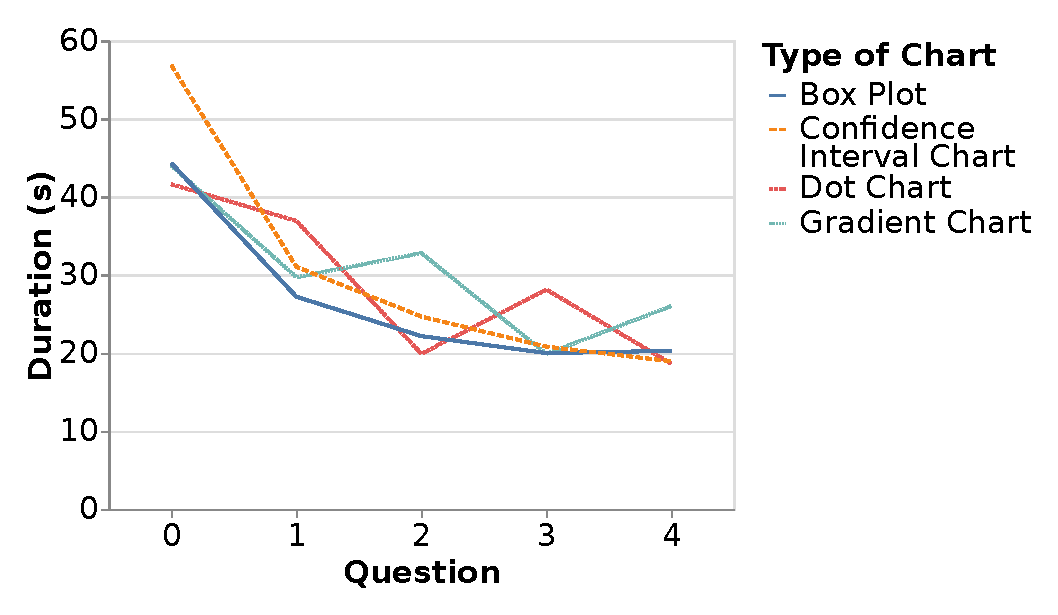
\includegraphics[width=0.6\textwidth]{duration_evo2}
  \caption{\label{figure:duration} Median time it took to answer each question
    for each of the types of chart.}
\end{figure}

After gathering all the answers from the participants, we calculated the
different metrics described in the previous section. Figure \ref{figure:errors}
displays the distribution of the reading error, the confidence, and the
perceived difficulty per type of chart.

It is interesting to note that, although we selected users with Masters level,
we did receive answers with probabilities above 1 or a probability as an
interval. This could be due to a misunderstanding of the chart's instructions or
a lack of statistical knowledge from those users and reinforces the fears
discussed in the introduction. We identified 9 users (3 for the natural
frequency chart, 4 for the confidence interval chart and 1 for the gradient
chart) from the whole set whose answers could not be used due to these reasons.

In the reading errors boxplot of figure \ref{figure:errors}, the worst chart in
terms of readability seems to be the gradient chart and the best is the natural
frequency time chart as it has a much lower reading error than the other charts.
As stated before, gradient charts are designed to showcase a general overview of
the distribution as they represent the evolution of the full range of
percentiles, however as shown by Cleveland et al. \cite{cleveland_graphical_1984}, the
color visual encoding is one of the worst forms of visual encoding and
limits the readability of the chart. Box plots and confidence interval charts
have similar reading errors: This is surprising as box plots display more
percentiles than the confidence interval. On the other hand, natural frequency
charts have a much lower readability error, and we can see how the use of
natural frequencies creates a more accurate reading experience.

Confidence and perceived difficulty boxplots (also shown in figure
\ref{figure:errors}) mirror the results in the reading error chart. It also
shows the superior ease of use of the natural frequency time chart: users
reported higher levels of confidence and lower levels of perceived difficulty
for this chart. Also, although the box plot and confidence interval have similar
reading errors, users perceive the confidence interval as more difficult to read
and are less confident with their readings. This can be explained by the simpler
nature of the confidence interval which only displays two percentiles and
requires users to estimate the position of the other percentiles only from those
two.

We can perform a statistical comparison of the reading errors of each chart with
the Kruskal-Wallis test \cite{krustal} and the Quade test
\cite{quade_rank_1967}. Both tests have a significantly low $p$-value (6.6e-10
and 5.6e-07) and confirm that the differences in reading errors are
statistically significant.

Table \ref{table:resultsperquestion} shows the error per question.
Interestingly, we can see that the open interval questions (3\ts{rd} and
5\ts{th} questions) had fewer errors than the other questions. The 4\ts{th}
question's error rate is high as the distribution of the target for that
question was concentrated in a relatively small interval and it was thus more
difficult to estimate the probability in that area.

We also recorded the time it takes to answer each of the questions as shown in
figure \ref{figure:duration}. We can see that the answering times are similar
for every chart and that this time decreases as the users answer questions. This
may be due to the fact that they are learning to use the charts and need less
time to answer the questions. However, due to the higher perceived difficulty,
we were expecting different answering times. Perhaps if we had increased the
number of questions, we would have seen a difference in the answering time due
to fatigue (or users simply quitting the test before its end).

\section{Conclusions}
\label{sec:concl}

As stated before, although the uncertainty visualization research field is rich
and presents an extensive list of visualization techniques, there are few
studies dealing with visualization techniques applied to time series, where the
evolution of uncertainty over time is relevant. After reviewing the existing
literature on the field, we found 3 visualization techniques we could apply to
this case: the gradient chart, the box plot, and the confidence interval charts.
Also, we applied frequency framing to design a fourth and novel way to visualize
uncertainty in time series. As the outcome probabilities are used to calculate
risks and rewards from decisions, we wanted to compare them against a predefined
set of metrics around the user's ability to estimate those probabilities. We
based our comparison on previous experiments on uncertainty visualizations, and
we devised a social experiment through Amazon Turk to evaluate the different
charts.

Although we could remark that the gradient chart, the box plot, or the
confidence interval charts are very good at providing an overall picture of the
uncertainty in the time series, we can see from this work that the application
of natural frequencies in an uncertainty chart does indeed provide better
numeric readability than any previous alternative. Natural frequencies do indeed
simplify the reading process as it simply consists of counting.

When using the natural frequency chart, there are several options like colors,
the number of circles, or the zoom level that are static. Further research would
be necessary to assess the effects of those attributes and check if providing
interactivity to modify those would improve or worsen the charts' readability.
Also, the charts were tested on the desktop computer: testing and optimizing the
charts for different form factors would also be interesting as it would provide
a new dimension for the research.

In conclusion, this type of chart should be promoted and used in real-world
applications as it helps decision-making when dealing with the uncertainty in
time series data.

\section{References}
\label{sec:ref}

\bibliography{refs}

\end{document}
